\section{Risultati Ottenuti}

I risultati ottenuti, che verranno dettagliatamente presentati 
nelle sezioni successive, possono essere riassunti in modo 
generale come risultati positivi, sia in termini di performance 
che di politiche applicate. In particolare, è possibile notare come 
il tempo generale della simulazione dipenda principalmente 
dall'applicazione del controllore e quindi dal calcolo della 
Neural ODE e tutte le operazioni correlate.

\begin{table}[htb]
    \centering
    \caption{Tempo Impiegato (HH:MM:SS)}
    \begin{tabular}{|p{2.57cm}||p{2.57cm}|p{2.57cm}|p{2.57cm}|p{2.57cm}|}
        \hline
        \multicolumn{5}{|c|}{Tipologia di Test} \\
        \hline
        & Nessun Intervento & Intervento Non Farmaceutico & Intervento Farmaceutico & Intervento Farmaceutico e Non \\
        \hline
        Singlerun (50 PdI) & 0:00:15 & 0:06:52 & 0:00:13 & 0:02:52 \\
        Ensemblerun (5 ripetizioni, 50 PdI) & 0:00:34 & 0:06:22 & 0:00:24 & 0:02:55 \\
        \hline
    \end{tabular}
\end{table}

\begin{table}[htb]
    \centering
    \caption{Tempo Impiegato (HH:MM:SS)}
    \begin{tabular}{|p{2.57cm}||p{2.57cm}|p{2.57cm}|p{2.57cm}|p{2.57cm}|}
        \hline
        \multicolumn{5}{|c|}{Tipologia di Test} \\
        \hline
        & Nodi Infetti Iniziali Variabili & Valore di Migrazione Variabile & Nodi della Rete Variabile & Copertura dei Nodi Variabile \\
        \hline
        Paramscan & 0:00:13 & 0:00:21 & 0:00:32 & 0:00:12 \\
        \hline
    \end{tabular}
\end{table}

Questi lunghi tempi di calcolo derivano dalla computazione delle 
contromisure non farmaceutiche applicate alla popolazione. 
Le contromisure farmaceutiche, se applicate con il giusto tempismo, 
oltre a contribuire notevolmente alla riduzione della diffusione 
della pandemia (vedi Figura \ref{fig:comparison_vax_1}, Figura 
\ref{fig:comparison_vax_2}, Figura \ref{fig:comparison_vax_3}, 
Figura \ref{fig:comparison_vax_4}), consentono una significativa 
riduzione dei tempi di calcolo.

\newpage

\subsection{Nessun Intervento}

Il seguente grafico (Figura \ref{fig:abm_no_intervent}) mostra l'andamento delle curve del modello quando questo viene eseguito senza alcuna tipologia di intervento. Questo andamento è rappresentato in modo cumulativo rispetto all'andamento dei singoli agenti, i quali possono mostrare comportamenti differenti tra loro.

\begin{minipage}{\linewidth}
    \centering
    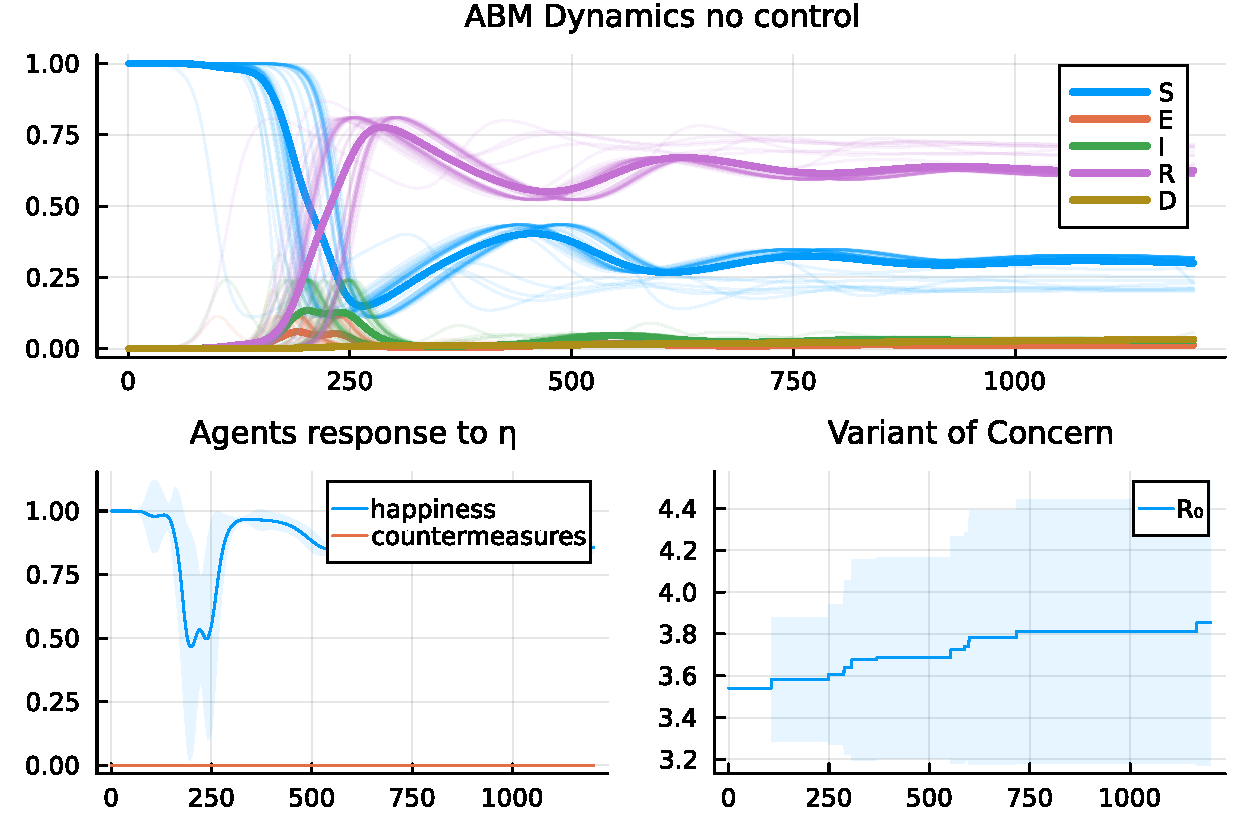
\includegraphics[width=\textwidth]{img/SocialNetworkABM_NO_CONTROL.pdf}
    \captionof{figure}{Grafico cumulativo del modello senza alcun tipo di intervento}
    \label{fig:abm_no_intervent}
\end{minipage}

Complessivamente, l'andamento del modello è simile a quello 
standard di un modello di tipo SEIR, con alcune variazioni 
dovute ai fattori di stocasticità intrinseci del modello. 
Il grafico mostra le traiettorie più comuni delle curve cumulative 
del modello, mettendo in evidenza i percorsi più frequenti.

Come è possibile notare, il numero di individui suscettibili 
diminuisce drasticamente a causa della rapida diffusione 
esponenziale del virus. Questo è accompagnato da una crescita 
altrettanto rapida del numero di individui guariti (recovered). 
Tuttavia, a causa della definizione delle condizioni per i guariti, 
questi individui non sono immuni alle varianti del virus, il che 
permette di modellare una possibile ciclicità dell'epidemia 
dovuta alla perdita di immunità della popolazione. 
Queste proprietà contribuiscono all'andamento ciclico delle curve. 
Inoltre, si nota che la curva associata all'andamento degli 
individui nella classe \emph{D} ha una crescita lineare, 
sebbene non molto evidente.

La curva associata alla variabile di "happiness" del modello, 
utilizzata per bilanciare la severità delle misure di controllo 
per evitare un ciclo insostenibile, mostra un comportamento 
piuttosto peculiare. Questo è principalmente dovuto alla 
definizione della funzione di controllo della felicità 
(vedi Figura \ref{fig:happinessf}). Inoltre, la curva tende 
ad oscillare in modo ciclico a causa della definizione delle 
misure di controllo.

In generale, il modello senza interventi mostra un'epidemia in 
rapida crescita seguita da periodi ciclici di riduzione della 
diffusione del virus.

\subsection{Intervento Non Farmaceutico}

Nel seguente grafico (Figura \ref{fig:abm_nonpharm_intervent}) è 
rappresentato l'andamento delle curve quando viene applicato un 
intervento non farmaceutico, come il distanziamento sociale, 
l'uso di maschere, ecc. L'obiettivo di questo tipo di intervento 
è quello di rallentare la diffusione del virus senza utilizzare 
farmaci o vaccini.

\begin{minipage}{\linewidth}
    \centering
    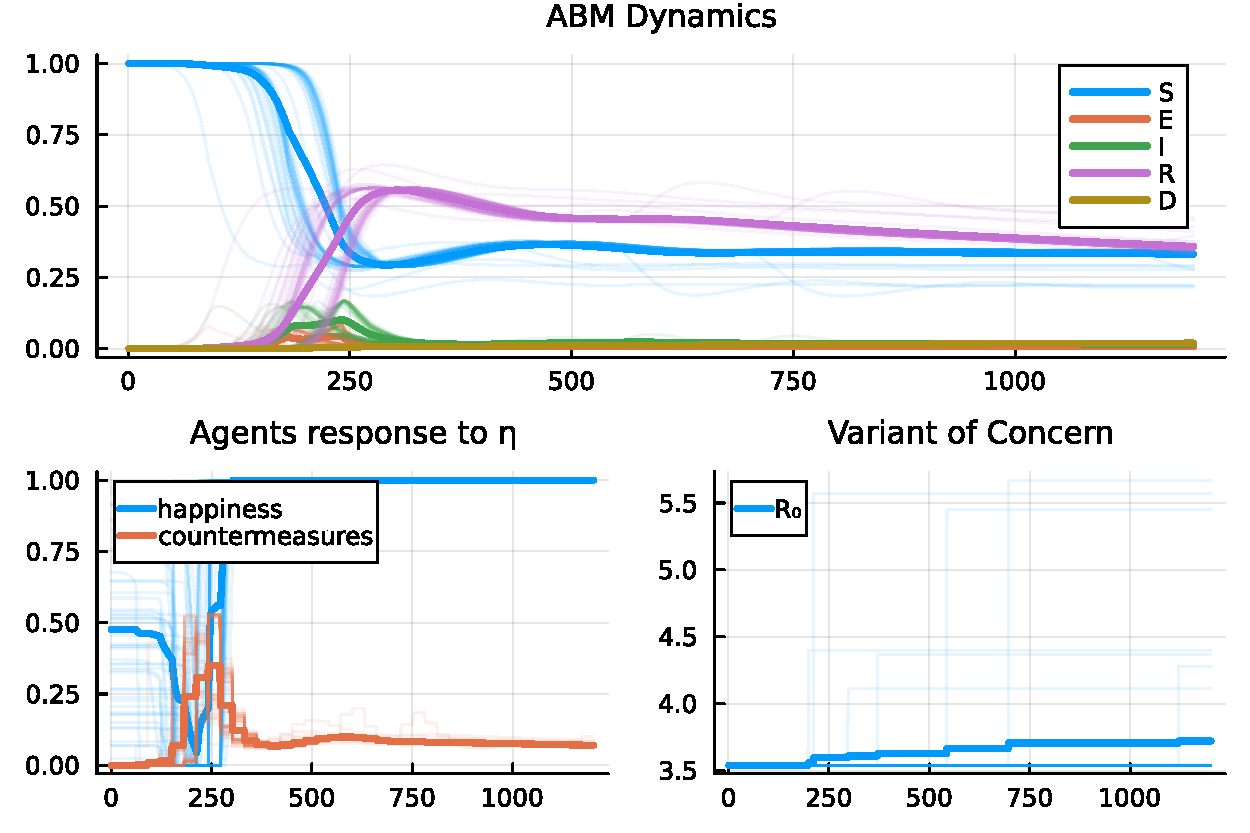
\includegraphics[width=\textwidth]{img/SocialNetworkABM_CONTROL.pdf}
    \captionof{figure}{Grafico cumulativo del modello con intervento non farmaceutico}
    \label{fig:abm_nonpharm_intervent}
\end{minipage}

Come si può vedere dal grafico, l'intervento non farmaceutico 
ha un impatto significativo sulla diffusione del virus. 
In particolare, il numero di individui suscettibili rimane 
più stabile nel tempo rispetto al caso senza interventi, e il 
picco dell'epidemia è notevolmente ridotto. Questo è dovuto 
all'efficacia delle misure di distanziamento sociale e al fatto 
che esse riducono il tasso di contatto tra gli individui infetti 
e suscettibili. Tuttavia, il numero di individui guariti è ancora 
ciclico a causa della perdita di immunità, e la curva di felicità 
mostra comunque oscillazioni dovute alle misure di controllo cicliche.

In generale, l'intervento non farmaceutico riesce a contenere 
l'epidemia e a ridurne l'entità, ma non riesce a eliminarla 
completamente.

\subsection{Intervento Farmaceutico}

Il seguente grafico (Figura \ref{fig:abm_pharm_intervent}) 
rappresenta l'andamento delle curve quando viene applicato un 
intervento farmaceutico, come la somministrazione di vaccini o 
farmaci antivirali. L'obiettivo di questo tipo di intervento è 
quello di ridurre significativamente la diffusione del virus e, 
idealmente, di eliminare l'epidemia.

\begin{minipage}{\linewidth}
    \centering
    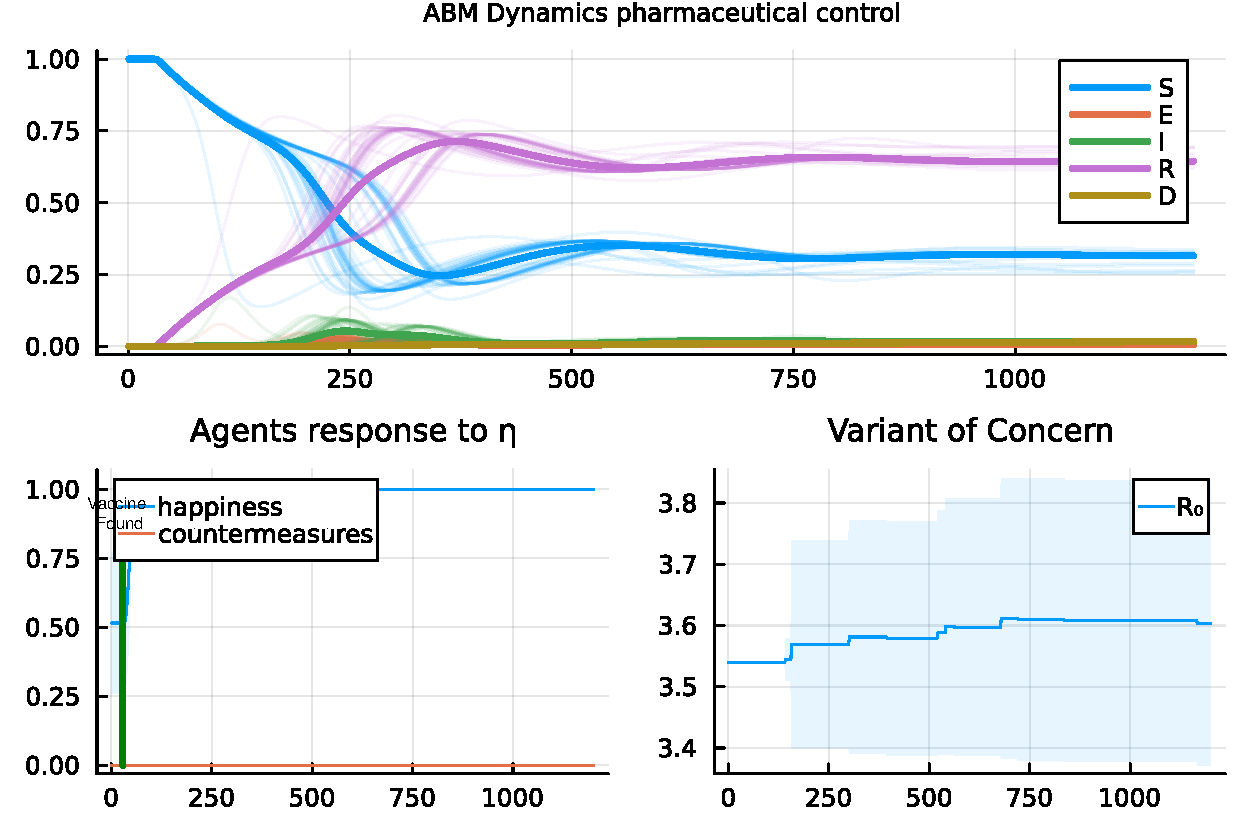
\includegraphics[width=\textwidth]{img/SocialNetworkABM_VACCINE.pdf}
    \captionof{figure}{Grafico cumulativo del modello con intervento farmaceutico}
    \label{fig:abm_pharm_intervent}
\end{minipage}

Come si può notare, l'intervento farmaceutico ha un impatto 
molto positivo sulla diffusione del virus. Il numero di individui 
suscettibili rimane stabile nel tempo, e l'epidemia viene rapidamente 
contenuta. Questo è dovuto alla somministrazione di farmaci o vaccini, 
che riducono la capacità di trasmissione del virus e proteggono gli 
individui suscettibili. Inoltre, il numero di individui guariti non 
mostra più l'andamento ciclico, poiché i soggetti guariti attraverso 
l'intervento farmaceutico acquisiscono immunità duratura.

La curva di felicità mostra ancora alcune oscillazioni dovute alle 
misure di controllo cicliche, ma queste oscillazioni sono meno 
pronunciate rispetto ai casi precedenti.

In generale, l'intervento farmaceutico è estremamente efficace nel 
contenere e ridurre l'epidemia.

\subsection{Intervento Farmaceutico e Non Farmaceutico}

Il seguente grafico (Figura \ref{fig:abm_combined_intervent}) 
rappresenta l'andamento delle curve quando vengono applicati sia 
un intervento farmaceutico che un intervento non farmaceutico. 
L'obiettivo di questa combinazione di interventi è quello di 
massimizzare la riduzione della diffusione del virus e di contenere 
l'epidemia in modo ottimale.

\begin{minipage}{\linewidth}
    \centering
    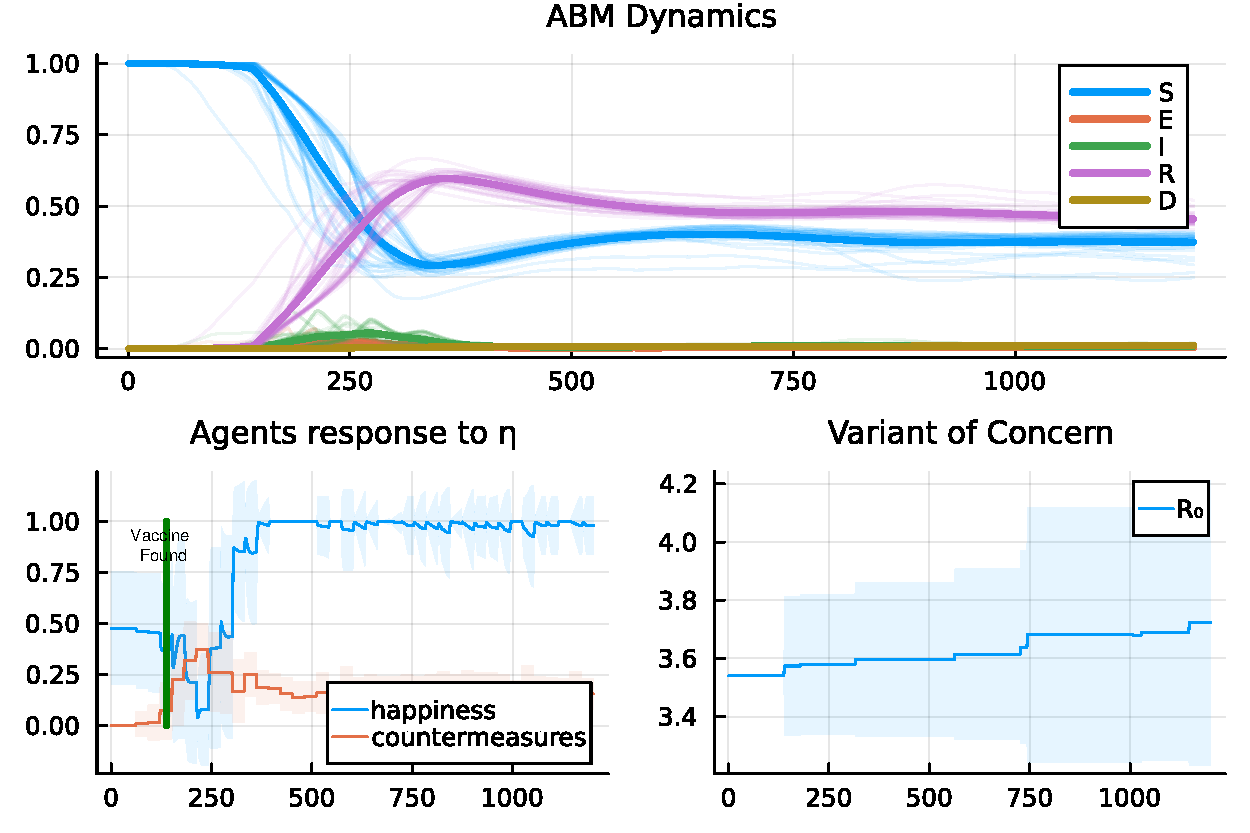
\includegraphics[width=\textwidth]{img/SocialNetworkABM_ALL.pdf}
    \captionof{figure}{Grafico cumulativo del modello con intervento farmaceutico e non farmaceutico combinato}
    \label{fig:abm_combined_intervent}
\end{minipage}

Come mostrato nel grafico, l'effetto combinato di intervento 
farmaceutico e non farmaceutico è estremamente efficace nel 
contenere l'epidemia. Il numero di individui suscettibili 
rimane stabile nel tempo, e l'epidemia viene rapidamente ridotta 
a livelli molto bassi. La curva di individui guariti mostra un 
aumento costante nel tempo, poiché l'intervento farmaceutico 
garantisce immunità duratura.

La curva di felicità mostra ancora alcune oscillazioni dovute 
alle misure di controllo cicliche, ma queste oscillazioni sono 
molto meno pronunciate rispetto ai casi precedenti.

In generale, la combinazione di intervento farmaceutico e non 
farmaceutico è altamente efficace nel contenere e ridurre 
l'epidemia in modo ottimale.

\section{Conclusione}

In conclusione, i risultati ottenuti dimostrano che l'applicazione 
di misure di controllo, sia farmaceutiche che non farmaceutiche, 
è estremamente efficace nel contenere e ridurre la diffusione del virus. 
L'intervento farmaceutico, in particolare, ha dimostrato di essere 
altamente efficace nel contenere l'epidemia e prevenire il ciclo 
insostenibile di infezioni. Tuttavia, l'intervento farmaceutico 
da solo potrebbe non essere sufficiente a eliminare completamente 
l'epidemia, mentre la combinazione di intervento farmaceutico e 
non farmaceutico offre una protezione ottimale.

I tempi di calcolo delle simulazioni sono significativamente 
influenzati dall'applicazione delle misure di controllo non 
farmaceutiche, ma questo è un compromesso necessario per ottenere 
risultati accurati e realistici. Inoltre, l'uso di misure di controllo 
cicliche può portare a oscillazioni nelle curve di felicità, 
ma queste oscillazioni sono gestibili.

In generale, il modello di simulazione dell'epidemia su una 
rete sociale offre una piattaforma utile per studiare gli effetti 
delle misure di controllo e per sviluppare strategie ottimali per 
la gestione delle epidemie.